\chapter{מ-Prompts למערכות סוכנים (From Prompts to Agent Systems)}
\section{2026 כנקודת מפנה: מ-helper לשכבה תפעולית}
במשך שנים נתפסו מודלי שפה ככלי עזר (helper) המסייע למשתמש האנושי לנסח טקסט, לסכם מסמך או להציע קטע קוד, כאשר האדם נשאר תמיד הגורם המבצע את הפעולה בפועל. שנת 2026 מסמנת נקודת מפנה (inflection point) משום שה-Agent חדל להיות נספח לממשק והופך לשכבה תפעולית (operational layer) בתוך אפליקציות ארגוניות. במקום שאדם יקרא תשובה ויעתיק אותה ידנית, ה-Agent קורא נתונים ממערכות פנימיות, מפעיל tools, כותב לבסיסי נתונים ומריץ תהליכים עסקיים מקצה לקצה. השינוי אינו טכנולוגי בלבד אלא ארכיטקטוני: ה-Agent ממוקם בנתיב הקריטי של זרימת העבודה, ולכן נדרשת ממנו אותה רמת אמינות, observability ו-validation המצופה מכל רכיב תוכנה תפעולי. ארגונים המטמיעים אותו מצפים כיום לא רק לתשובה משכנעת, אלא להתנהגות צפויה, ניתנת לניטור ולחזרה (reproducible). מכאן נובע הצורך במסגרות כמו CrewAI, המגדירות במפורש Agent, Task, Crew ו-Process כדי לתחום אחריות ולאפשר פיקוח. המעבר משכבת עזר לשכבה תפעולית מחייב מהנדסים לתפוס את ה-Agent לא כקסם גנרטיבי, אלא כרכיב מערכת מתוזמר בעל קלט מוגדר, פלט מאומת והקשר (Context) מבוקר. זוהי המהפכה שהפרק הזה בא לתאר ולבסס.

\section{מדוע prompt בודד וארוך נכשל}
הפיתוי הראשוני בבניית מערכת מבוססת מודל שפה הוא לדחוס את כל הדרישות ל-prompt בודד וארוך: להסביר את המשימה, לצרף את כל הנתונים, לפרט את הכללים ולקוות שהמודל יפיק תוצאה שלמה במכה אחת. בפועל גישה זו קורסת ככל שמורכבות המשימה גדלה. ראשית, חסר planning: המודל מתבקש להחזיק בו-זמנית את התכנון, הביצוע והבדיקה, ולכן נוטה לדלג על שלבים או לסתור את עצמו. שנית, חסר memory: בלא מנגנון זיכרון מפורש כל אינטראקציה מתחילה מאפס, ומידע שנצבר בצעד קודם נשמט. שלישית, חסרים tools: מודל מבודד אינו יכול לקרוא קובץ עדכני, להריץ חישוב מדויק או לפנות ל-API חיצוני, ולכן הוא ממציא עובדות במקום לאחזר אותן. ומעל הכל חסרה שכבת בקרה, ה-Harness, שתפקידה לתזמר את הצעדים, לאכוף סכמות, להפעיל validation על כל פלט ולמנוע משגיאה בצעד אחד לזהם את כל התהליך. ה-Harness הוא שהופך אוסף קריאות למודל למערכת תפעולית אמינה: הוא קובע סדר, מטפל בכשלים, מספק observability ומאפשר חזרתיות. לפיכך prompt בודד אינו נכשל בשל חולשת המודל, אלא בשל היעדר ארכיטקטורה סביבו. המסקנה היא שמערכת סוכנים רצינית דורשת הפרדה מפורשת בין תכנון, זיכרון, כלים ובקרה.

\section{תזת הספר: פירוק לצעדים תחומים, ניתנים לבדיקה ולשליטה}
התזה המרכזית של ספר זה היא שכדי להפוך משימה גנרטיבית רחבה למערכת אמינה יש לפרק אותה לצעדים תחומים (bounded), ניתנים לבדיקה (inspectable) וניתנים לשליטה (controllable). במקום לבקש מן המודל להפיק תוצר ענק במכה אחת, אנו מגדירים שרשרת של Task יחידות, שלכל אחת קלט מוגדר, פלט בעל סכמה ברורה ואחריות מצומצמת. צעד תחום פירושו שהיקפו ידוע מראש ושאפשר להעריך את הצלחתו במנותק מן השאר. צעד ניתן לבדיקה פירושו שהפלט שלו אינו קופסה שחורה אלא artifact שאפשר לפתוח, לאמת מול validation ולהשוות לציפייה, כך ש-observability נבנית לתוך המערכת ולא מודבקת עליה בדיעבד. צעד ניתן לשליטה פירושו שה-Harness יכול לעצור, לחזור על צעד, להחליף Context או לחסום פלט שאינו עומד בכללים, בטרם יזרום הלאה. כך, למשל, הפקת מסמך LaTeX מורכב הופכת לרצף של צעדים, שכל אחד מהם מיוצר ונבדק בנפרד, במקום ניסיון יחיד ושביר. גישה זו ממירה את אי-הוודאות הגנרטיבית במבנה הנדסי: ה-Agent עדיין מספק את היצירתיות, ואילו ה-Process וה-Crew מספקים את המשמעת. שאר הספר מפתח עיקרון זה לכדי דפוסי תכן מעשיים, ומראה כיצד בונים מערכות סוכנים שניתן לסמוך עליהן בסביבה תפעולית אמיתית.

לקריאה נוספת בנושאי פרק זה, ראו \cite{crewai_docs}.

\section{איורים, טבלה ונוסחה}
פרק זה מסתמך על תיעוד ה-framework \cite{crewai_docs}.

\begin{figure}[h]
\centering
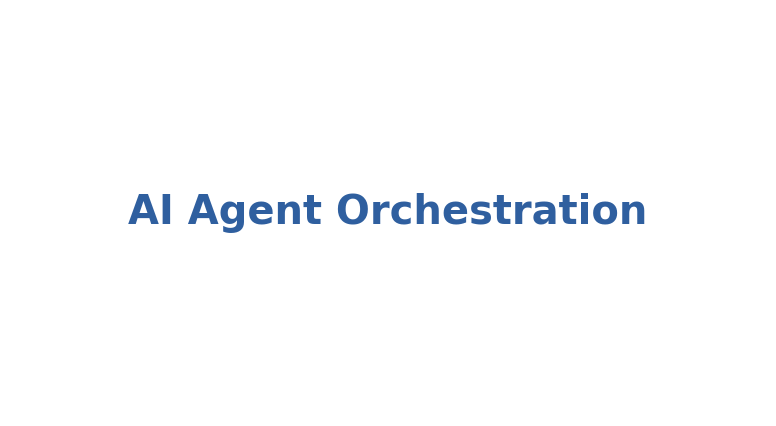
\includegraphics[width=0.6\textwidth]{assets/course_concept_image.png}
\caption{Illustration of course concept.}
\end{figure}

\begin{figure}[h]
\centering
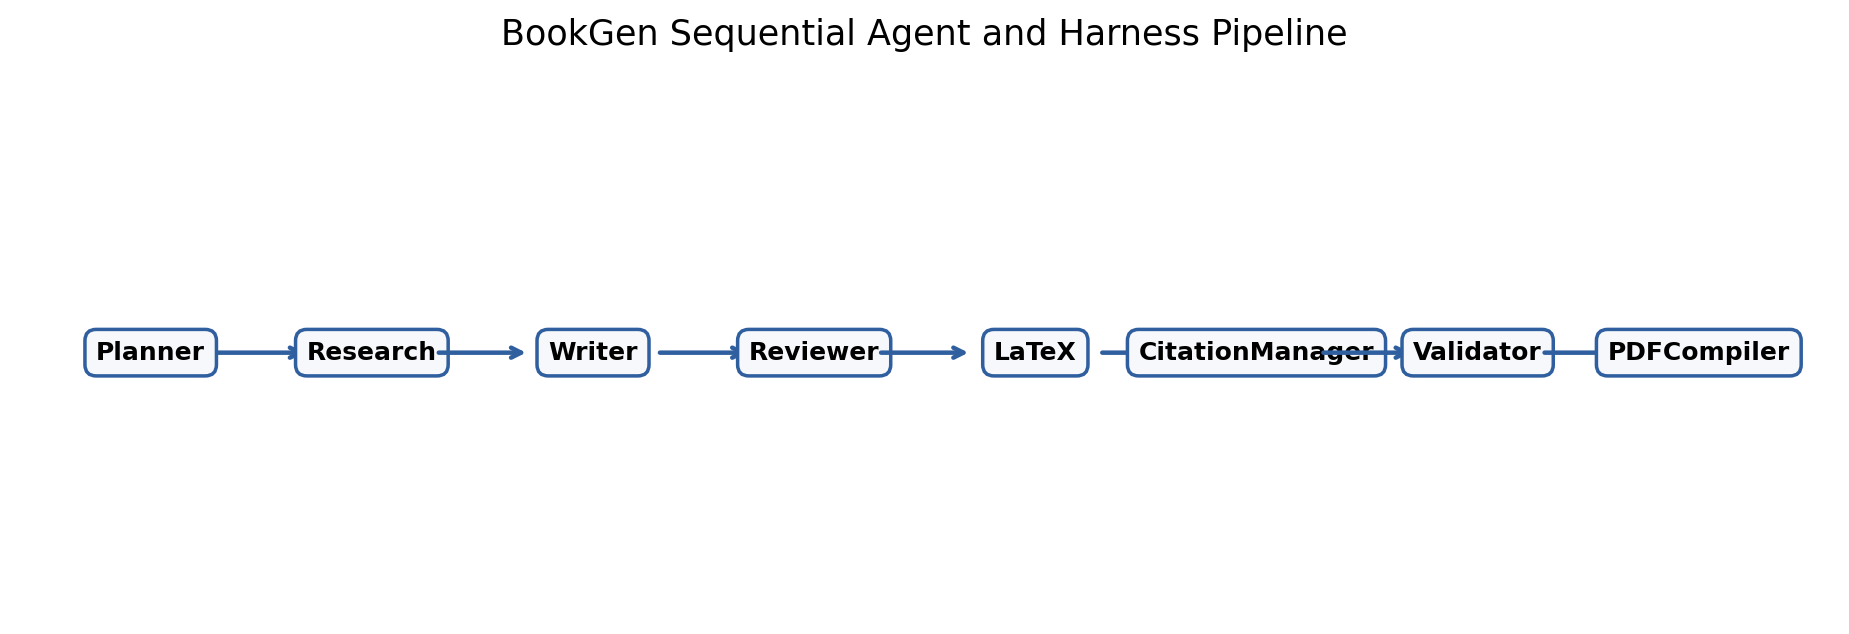
\includegraphics[width=0.9\textwidth]{assets/agent_pipeline_graph.png}
\caption{Graphical representation of the agent pipeline.}
\end{figure}

\begin{table}[h]
\centering
\small
\begin{tabular}{p{0.18\linewidth}p{0.25\linewidth}p{0.43\linewidth}}
\toprule
Metric & מה הוא מודד & שימוש טקטי \\
\midrule
xG & איכות בעיטות & לבדוק אם הקבוצה יוצרת מצבים טובים \\
PPDA & עוצמת לחץ & להשוות לחץ גבוה מול לחץ פסיבי \\
Field tilt & שליטה בשליש היריב & לזהות החזקת כדור מסוכנת \\
Progressive passes & קידום כדור & למדוד שבירת קווי הגנה \\
Pass network & קשרים בין שחקנים & לזהות מוקדי בנייה ובידוד שחקנים \\
\bottomrule
\end{tabular}
\normalsize
\caption{השוואה בין מדדים מרכזיים בניתוח כדורגל.}
\end{table}
\begin{equation}
Q = \sum_{i=1}^{n} w_i \cdot s_i
\end{equation}
\section{מעבר דו-כיווני בין עברית לאנגלית}
הטקסט הראשי כתוב בעברית (RTL), ומונחים טכניים נשמרים באנגלית (LTR). לדוגמה, משפט שלם באנגלית:
\begin{english}
The system combines planning, research, writing, and review under a deterministic harness.
\end{english}
כאן מודגם המעבר התקין בין כיוון הכתיבה מימין-לשמאל לכיוון משמאל-לימין.
